\documentclass[aspectratio=1610, polish]{beamer} 
% Jeśli chcesz otrzymać prezentację w języku polskim, to, powyżej, zamień „english” na „polish”
\usepackage{babel}
\makeatletter
\@ifclasswith{beamer}{polish}{
	\usepackage{polski}
}
\makeatother
\usepackage[utf8]{inputenc}
\usepackage{listings} % We want to put listings
% \usepackage{minted}   % We want to put listings

\mode<beamer>{ 	% In the 'beamer' mode
	\hypersetup{pdfpagemode=FullScreen}         % Enable Full screen mode
	\usetheme[parttitle=rightfooter, nosidebar, margins=1em]{AGH}       % Show part title in right footer
	%\usetheme[nosidebar]{AGH}                  % Do not show sidebar on non-title slides
	% \usetheme[nosidebar, margins=1em]{AGH}     % Do not show sidebar on non-title slides and set both margins (left / right) to 1em
	%\usetheme[dark]{AGH}                       % Use dark background
	%\usetheme[dark, parttitle=leftfooter]{AGH} % Use dark background and show part title in left footer
}
\mode<handout>{	% In the 'handout' mode
	\hypersetup{pdfpagemode=None}		
	\usepackage{pgfpages}
	\pgfpagesuselayout{4 on 1}[a4paper,border shrink=5mm,landscape]	% Show 4 slides on 1 page
	\pgfpageslogicalpageoptions{1}{border code=\pgfusepath{stroke}}
	\pgfpageslogicalpageoptions{2}{border code=\pgfusepath{stroke}}
	\pgfpageslogicalpageoptions{3}{border code=\pgfusepath{stroke}}
	\pgfpageslogicalpageoptions{4}{border code=\pgfusepath{stroke}}
  	\usetheme{boxes}
  	\addheadbox{structure}{\quad\insertpart\hfill\insertsection\hfill\insertsubsection\qquad}          % Content of header
 	\addfootbox{structure}{\quad\insertshortauthor\hfill\insertframenumber\hfill\insertsubtitle\qquad} % Content of footer
}

\AtBeginPart{ % At begin part: display its name
	\frame{\partpage}
} 
\author[Beata Trzpil-Jurgielewicz]{mgr inż. Beata \textsc{Trzpil-Jurgielewicz}
\newline 
promotorzy:
\newline
prof. dr hab. inż. Władysław \textsc{Dąbrowski} 
\newline 
dr inż. Paweł \textsc{Hottowy}}
\date{}
\iflanguage{polish}
{
	\title[]{Opracowanie wielokanałowego układu scalonego w technologii CMOS do rejestracji aktywności neuronalnej oraz jego aplikacja w funkcjonalnych badaniach mózgu
	}
	% \institute[AGH]{
	% 		\inst{1}Instytut Informatyki\newline
	% 		ul. Kawiory 21\newline
	% 		30-055 Kraków\newline
	% 		\url{http://www.icsr.agh.edu.pl/~polak/}
	% 	\and
	% 		\inst{2}Druga afiliacja
 	% }
}{
	\title{---}
	% \institute[AGH]{
	% 		\inst{1}Institute of Computer Science\newline
	% 		Kawiory 21 Street\newline
	% 		30-055 Kraków\newline
	% 		Poland\newline
	% 		\url{http://www.icsr.agh.edu.pl/~polak/}
	% 	\and
	% 		\inst{2}Second affiliation
	% }
}
%%%%%%%%%%% Configuration of the listings package %%%%%%%%%%%%%%%%%%%%%%%%%%
% Source: https://en.wikibooks.org/wiki/LaTeX/Source_Code_Listings#Using_the_listings_package
%%%%%%%%%%%%%%%%%%%%%%%%%%%%%%%%%%%%%%%%%%%%%%%%%%%%%%%%%%%%%%%%%%%%%%%%%%%%
\lstset{ %
  backgroundcolor=\color{white},   % choose the background color
  basicstyle=\footnotesize,        % the size of the fonts that are used for the code
  breakatwhitespace=false,         % sets if automatic breaks should only happen at whitespace
  breaklines=true,                 % sets automatic line breaking
  captionpos=b,                    % sets the caption-position to bottom
  commentstyle=\color{green},      % comment style
  deletekeywords={...},            % if you want to delete keywords from the given language
  escapeinside={\%*}{*)},          % if you want to add LaTeX within your code
  extendedchars=true,              % lets you use non-ASCII characters; for 8-bits encodings only, does not work with UTF-8
  frame=single,	                   % adds a frame around the code
  keepspaces=true,                 % keeps spaces in text, useful for keeping indentation of code (possibly needs columns=flexible)
  keywordstyle=\color{blue},       % keyword style
  morekeywords={*,...},            % if you want to add more keywords to the set
  numbers=left,                    % where to put the line-numbers; possible values are (none, left, right)
  numbersep=5pt,                   % how far the line-numbers are from the code
  numberstyle=\tiny\color{gray},   % the style that is used for the line-numbers
  rulecolor=\color{black},         % if not set, the frame-color may be changed on line-breaks within not-black text (e.g. comments (green here))
  showspaces=false,                % show spaces everywhere adding particular underscores; it overrides 'showstringspaces'
  showstringspaces=false,          % underline spaces within strings only
  showtabs=false,                  % show tabs within strings adding particular underscores
  stepnumber=2,                    % the step between two line-numbers. If it's 1, each line will be numbered
  stringstyle=\color{cyan},        % string literal style
  tabsize=2,	                   % sets default tabsize to 2 spaces
  title=\lstname,                  % show the filename of files included with \lstinputlisting; also try caption instead of title
                                   % needed if you want to use UTF-8 Polish chars
  literate={ą}{{\k{a}}}1
           {Ą}{{\k{A}}}1
           {ę}{{\k{e}}}1
           {Ę}{{\k{E}}}1
           {ó}{{\'o}}1
           {Ó}{{\'O}}1
           {ś}{{\'s}}1
           {Ś}{{\'S}}1
           {ł}{{\l{}}}1
           {Ł}{{\L{}}}1
           {ż}{{\.z}}1
           {Ż}{{\.Z}}1
           {ź}{{\'z}}1
           {Ź}{{\'Z}}1
           {ć}{{\'c}}1
           {Ć}{{\'C}}1
           {ń}{{\'n}}1
           {Ń}{{\'N}}1
}
\usepackage{booktabs}
\usepackage{siunitx}
\sisetup{locale = PL,
         exponent-product=\ensuremath{\times}}
\graphicspath{{../PhD_Thesis_BTJ/Figures/}}
% \graphicspath{{../BTJ_Thesis/Figures/}}

\usepackage{caption}
\usepackage{subcaption}
\usepackage{tabularray}

\usepackage[most]{tcolorbox}    	% for COLORED BOXES (tikz and xcolor included)
\usepackage{ninecolors}
\selectcolormodel{rgb}
\definecolor{main}{HTML}{1F77B4}    % setting main color to be used
\definecolor{sub}{HTML}{cde4ff}     % setting sub color to be used
\definecolor{deepblue}{HTML}{1F77B4}
\definecolor{deepred}{HTML}{D92728}
\definecolor{lightred}{HTML}{D98789}
\definecolor{deepgreen}{HTML}{2CA02C}

\tcbset{
    sharp corners,
    colback = white,
    before skip = 0.2cm,    % add extra space before the box
    after skip = 0.5cm      % add extra space after the box
}  

\newtcolorbox{boxR}{
    enhanced, % for a fancier setting,
    boxrule = 0pt, % clearing the default rule
    borderline = {0.75pt}{0pt}{deepred}, % outer line
    borderline = {0.75pt}{2pt}{lightred}, % inner line
    % title = sda
}

%%%%%%%%%%% Configuration of the minted package %%%%%%%%%%%%%%%%%%%%%%%%%%
% \setminted[C++]{frame=single,linenos}

%%%%%%%%%%%%%%%%%
\begin{document}
\maketitle


% \part{Tematyka pracy}
\begin{frame}{Plan prezentacji}
	\tableofcontents%[pausesections]
\end{frame}
\section{Systemy do rejestracji aktywności elektrycznej żywych tkanek nerwowych}
\section{Projekt liniowego pseudo-rezystora w zakresie \si{\giga\ohm}}
\section{Operacyjny wzmacniacz transkonduktancyjny}
\section{Weryfikacja elektroniczna i neurofizjologiczna układu scalonego HiFiNeuroPre}

\part{Tematyka pracy}
\begin{frame}{Cele pracy}

    \begin{alertblock}{}
        Celem projektu przedstawionego w niniejszej pracy było opracowanie i weryfikacja koncepcji przedwzmacniacza dedykowanego do wielokanałowej sondy neuronalnej umożliwiającej rejestrację aktywności neuronalnej mózgu.
    \end{alertblock}

    \begin{block}{Główne zadania}
        \begin{itemize}
            \item Kompleksowa analiza zniekształceń nieliniowych we wzmacniaczach neuronalnych
            \item Optymalizacja kluczowych parametrów przedwzmacniaczy neuronalnych
            \item  Projekt układu scalonego, obwodu drukowanego oraz systemu akwizycji danych
            \item Wykonanie testów elektronicznych oraz analiza parametrów i charakterystyk opracowanego układu scalonego
            \item Weryfikacja funkcjonalności opracowanego przedwzmacniacza  w eksperymentach neurobiologicznych i analiza zebranych danych
        \end{itemize}
    \end{block}

    
\end{frame}

\begin{frame}{Zakresy amplitud i częstotliwości sygnałów neuronowych w różnych technikach rejestracji}
    \begin{columns}
        \column{.48\textwidth}
        \vspace{-2em}

        \begin{figure}[H]
            \includegraphics[scale=0.2]{ch1/brain.jpg}
          \end{figure}

          \begin{block}{Metody rejestracji}
            \begin{itemize}
                {\renewcommand\normalsize{\small}%
                \normalsize
                \item LFP -- Local Field Potential
                \item AP --  Action Potential
                \item ECoG -- Electrocorticography
                \item EEG -- Electroencephalography
                }
            \end{itemize}
        \end{block}


        \column{.48\textwidth}
        \vspace{-2em}

        \begin{figure}[H]
            \centering
            \includegraphics[scale=1.0]{ch1/lfp_ap_spectrum}  
            \end{figure}	
    \end{columns}
    
\end{frame}

\begin{frame}{Kierunki rozwoju współczesnych systemów pomiarowych i matryc mikroelektrodowych}
   
    \begin{columns}
    \column{.55\textwidth}

    \begin{block}{Techniki pomiarowe wewnątrz i \\
        zewnątrzkomórkowe w neurobiologii}
        \begin{itemize}
            \item różne amplitudy sygnałów
            \item inwazyjność badań
            \item obszar badań 
        \end{itemize}
    \end{block}
    \column{.4\textwidth}
    \vspace{-3em} %5mm vertical space

        \begin{columns}
        \column{.5\textwidth}
        \begin{figure}[H]
            \includegraphics[scale=0.13]{ch2/masm64Dsharp.png}
        \end{figure}

        \column{.5\textwidth}
            \begin{figure}[H]
                \includegraphics[scale=0.13]{ch2/utahArr.png}
            \end{figure}
        \end{columns}
    \end{columns}

    \begin{columns}

        \column{.55\textwidth}
        % \vspace{-3em} %5mm vertical space

        \begin{figure}[H]
            \includegraphics[scale=0.45]{ch1/intra-extra.png}  
        \end{figure}

        \column{.4\textwidth}
        \vspace{-2em} %5mm vertical space
        \begin{figure}[H]
                % \includegraphics[scale=0.25]{ch1/ap.png}
            \includegraphics[scale=0.25]{ch2/neuropixel10.png}  
        \end{figure}


    \end{columns}


    
\end{frame}

% \begin{frame}{Kierunki rozwoju współczesnych systemów pomiarowych i matryc mikroelektrodowych}
%     \vspace{-5mm} %5mm vertical space

%     \begin{columns}[t]
%         \column{.3\textwidth}
%         \begin{figure}[H]
%             \includegraphics[scale=0.35]{ch2/neuropixel10.png}  
%         \end{figure}

%         \column{.3\textwidth}
%         \begin{figure}[H]
%             \includegraphics[scale=0.35]{ch2/argo.jpeg}  
%         \end{figure}

%         \column{.35\textwidth}
%         \begin{figure}[H]
%             \includegraphics[scale=0.2]{ch2/masm64Dsharp.png}
%         \end{figure}

%         \begin{figure}[H]
%             \includegraphics[scale=0.25]{ch2/utahArr.png}
%         \end{figure}

%     \end{columns}


% \end{frame}





\begin{frame}{Kanał rejestracji neuronowej z wykorzystaniem mikroelektrod zewnątrzkomórkowych}
\vspace{-1em}
    \begin{columns}
        \column{.48\textwidth}
        \begin{figure}[H]
            \centering
            \includegraphics[scale=0.25]{ch2/chemNeuroInterface.png} 

        \end{figure}
        \begin{figure}[H]
            \centering
            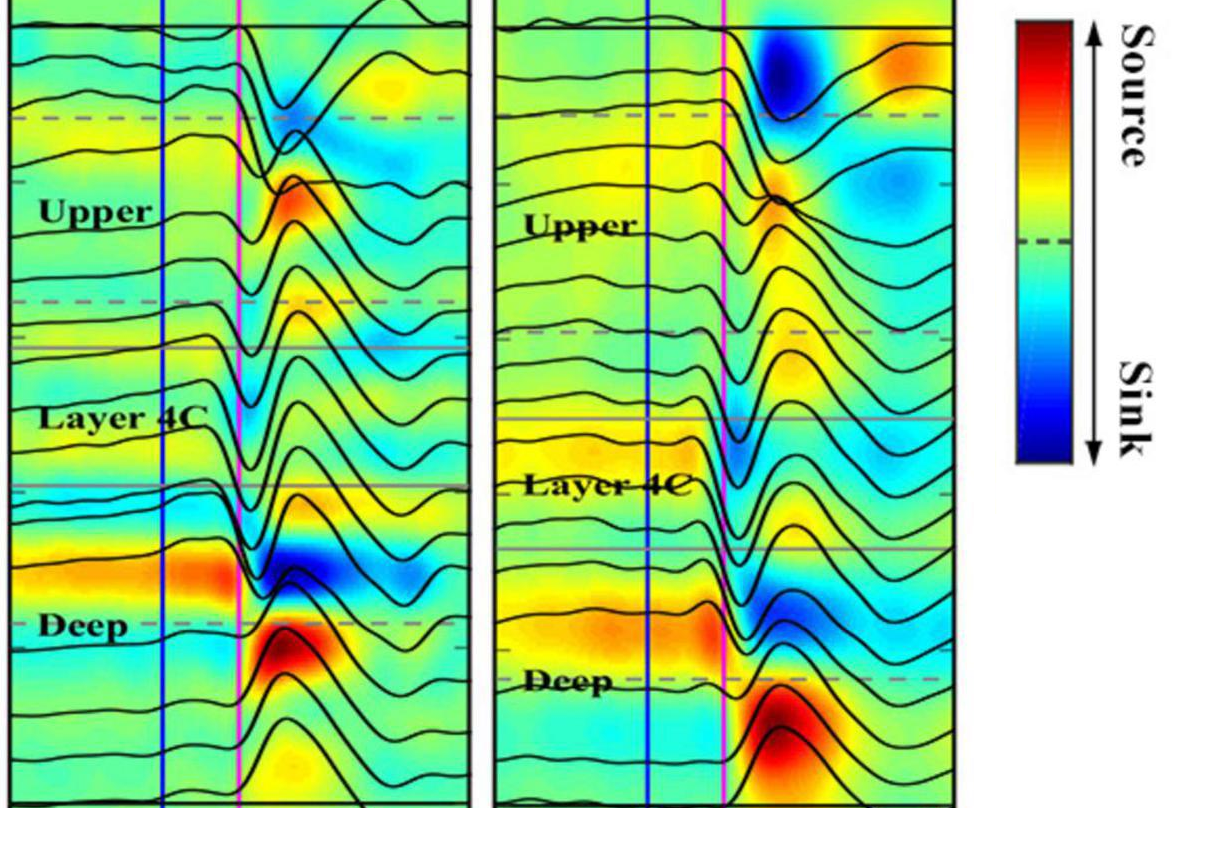
\includegraphics[scale=0.25]{ch1/lfp.png} 

          \end{figure}

        \column{.48\textwidth}
        \begin{block}{Wymagania stawiane interfejsom neuroelektronicznym umożliwiającym rejestrację sygnałów LFP i AP}
            \begin{itemize}
                \item Stałe napięcie na styku elektrody -- do $\SIrange{1}{2}{\volt}$ 
                \item Szumy $<\SI{10}{\micro\volt}$ dla pasma LFP i AP
                \item Liniowość rejestrowanego sygnału
                \item Pobór mocy -- limit ogrzewania tkanki mózgowej --  mniej niż  $\SI{1}{\degreeCelsius}$ 
                \item Zróżnicowane sygnały: amplituda do $\SI{10}{\milli\volt_{pp}}$ dla LFP i od  $\SI{50}{\micro\volt}$ dla AP
                \item Skalowalność -- tysiące kanałów dla przyszłych systemów
            \end{itemize}
        \end{block}
        % Schemat typowego kanału rejestracji neuronowej i modelu elektrycznego interfejsu tkanka-mikroelektroda: 
        % $Z_{CPA}$ -- element o stałej fazie, 
        % $R_{CT}$ -- rezystancja dla przepływającego prądu przez elektrodę,  
        % $R_{SP}$ -- rezystancja rozproszona elektrolitu, 
        % $V_{HC}$ -- potencjał w interfejsie elektroda -- tkanka. 
 
    \end{columns}
\end{frame}


% \begin{frame}{Sprzężenie zmiennoprądowe}
%     \begin{columns}
%         \column{.48\textwidth}

%     \begin{figure}[H]
%         \centering
%         \includegraphics[scale=0.75]{ch2/conceptAC_Harrison.pdf} 
%     \end{figure}
%     \column{.48\textwidth}
%     \begin{alertblock}{Wyzwania zwiazane z sprzęzeniem AC}
%         \begin{itemize}
%             \item Niska dolna częstotliwość graniczna rzędu~$\SI{\sim 1}{\hertz}$ 
%             \item Pojemności w technologi CMOS są rzędu $\SI{}{\femto\farad\per\micro\metre\squared}$
%             \item Rezystancja sprzężenia zwrotnego w zakresie $\SI{}{\tera\ohm}$
%         \end{itemize}
%     \end{alertblock}
%     \begin{exampleblock}{Zalety}
%         \begin{itemize}
%             \item Usunięcie składowej stałej od elektrody niezależnie od jej wartości
%             \item Wydajność szumowa i poboru mocy
%         \end{itemize}
%     \end{exampleblock}
% \end{columns}

% \end{frame}



% \begin{frame}{Sprzężenie stałoprądowe}
%     \begin{columns}
%         \column{.48\textwidth}
%         \begin{figure}[H]
%             \centering
%             \includegraphics[scale = 0.5]{ch2/dc_coupling.pdf}
%         \end{figure}

%     \column{.48\textwidth}
%     \begin{alertblock}{Wyzwania zwiazane z sprzęzeniem DC}
%         \begin{itemize}
%             \item Duża wrażliwość na offset
%             \item Pobór mocy
%         \end{itemize}
%     \end{alertblock}
%     \begin{exampleblock}{Zalety}
%         \begin{itemize}
%             \item Brak konieczności używania dużych rezystancji w pętli sprzężenia zwrotnego
%         \end{itemize}

%         \begin{figure}[H]
%             \centering
%             \includegraphics[scale=0.5]{ch2/dc-integrator.pdf} 
%         \end{figure}

%     \end{exampleblock}
% \end{columns}

% \end{frame}

\begin{frame}{Sprzężenie zmiennoprądowe i stałoprądowe}
    

    \begin{columns}
        \column{.55\textwidth}
        \vspace{-1em} %5mm vertical space

        \begin{figure}[H]
            \centering
            \includegraphics[scale=0.5]{ch2/conceptAC_Harrison.pdf} 
        \end{figure}
        \vspace{-2em} %5mm vertical space

        {\renewcommand\normalsize{\small}%
        \normalsize
    
        % \begin{alertblock}{Wyzwania zwiazane z sprzęzeniem AC}
    %5mm vertical space
    
        % \begin{exampleblock}{Zalety}
        % \begin{exampleblock}{Sprzężenie zmiennoprądowe}
        \begin{exampleblock}{}

            \begin{itemize}
                \item Całkowite usunięcie napięcia stałego na elektrodzie 
                \item Konieczność implementacji filtru górnoprzepustowego z dolną częstotliwością graniczną rzędu~$\SI{\sim 1}{\hertz}$ 
                \item Ograniczenia na pojemności kondensatorów w technologii CMOS ~pF $\sim\SI{}{\pico\farad}$
                \item  Wymagane rezystancje  $\sim\SI{}{\tera\ohm}$
            \end{itemize}
        \end{exampleblock}
    
        }


        \column{.43\textwidth}
        \vspace{-3em} %5mm vertical space

        \begin{figure}[H]
            \hspace{-2em} %5mm vertical space
            \includegraphics[scale = 0.48]{ch2/dc_coupling.pdf}
        \end{figure}


    {\renewcommand\normalsize{\small}%
    \normalsize
    % \begin{alertblock}{Wyzwania zwiazane z sprzęzeniem DC}
    \vspace{-1em} %5mm vertical space

    % \begin{alertblock}{Sprzężenie stałoprądowe}
        \begin{alertblock}{}

        \begin{itemize}
            \item Alternatywne podejście do eliminacji składowej stałej napięcia na styku elektrody i tkanki
        \end{itemize}
    \end{alertblock}
    }

    \end{columns}

\end{frame}


\part{Liniowy pseudo-rezystor}


% \begin{frame}{Podstawowe rozwiązania psuedo-rezystorów}


%         \begin{figure}[H]
%             \centering
%             \includegraphics[scale = 0.6]{ch2/ntpr.pdf}

%         \end{figure}
%         \vspace{-5mm} %5mm vertical space
%         % Różne topologie pseudo-rezystorów z niekontrolowaną wartością rezystancji zaimplementowane w przedwzmacniaczu ze sprzężeniem zmiennoprądowym.        
%         \begin{alertblock}{Wady}
%             \begin{itemize}
%                 \item stała rezystancja 
%                 \item brak możliwości regulacji częstotliwości granicznej
%             \end{itemize}
%         \end{alertblock}



% \end{frame}

% \begin{frame}{Podstawowe rozwiązania psuedo-rezystorów - regulowana wartość rezystancji}
%     \begin{block}{}
%         Regulacja częstotliowści granicznej
%     \end{block}

%     \begin{columns}
%         \column{.58\textwidth}
%         \hspace{-10mm} %5mm vertical space
%         \begin{figure}[H]

%             \includegraphics[scale = 0.6]{ch2/tpr.pdf}

%         \end{figure}
%         \column{.35\textwidth}
%         % Różne topologie pseudo-rezystorów z kontrolowaną wartością rezystancji zaimplementowane w przedwzmacniaczu ze sprzężeniem zmiennoprądowym.
%         \vspace{-5mm} \begin{alertblock}{}
%         Zmieniające się napięcie panujące pomiędzy bramką a źródłem tranzystora w zależności od sygnału wejściowego
%         \end{alertblock}
%         \vspace{5mm} 
%         \begin{exampleblock}{}
%             Zachowanie stałego napięcia pomiędzy bramką, a źródłem niezależnie od sygnału wejsciowego 

%         \end{exampleblock}
%     \end{columns}


% \end{frame}


\begin{frame}{Podstawowe rozwiązania psuedo-rezystorów}
    \vspace{-1em}
    \begin{block}{}
        Zastosowanie tranzystorów jako elementów rezystancjach, zwanych pseudo-rezystorami, jest powszechną praktyką w projektowaniu obwodów analogowych dla przypadków, w których bierne rezystory nie są odpowiednie ze względu na wartości wymaganych rezystancji lub powierzchnie takich elementów. 
       \end{block}
    \begin{columns}
        \column{.48\textwidth}
        \vspace{-2em}
        \begin{figure}[H]
            \includegraphics[scale = 0.4]{ch2/ntpr.pdf}
        \end{figure}
        \begin{alertblock}{}
            brak możliwości regulacji wartości rezystancji
        \end{alertblock}



        \column{.48\textwidth}
        \begin{figure}[H]
            \includegraphics[scale = 0.4]{ch2/tpr.pdf}
        \end{figure}
        \vspace{-1em}
        \begin{exampleblock}{}
            możliwość regulacji wartości rezystancji za pomocą modyfikacji napięcia panującego na bramce tranzystora
        \end{exampleblock}

    \end{columns}
\end{frame}








% \begin{frame}{Analiza stałoprądowa}

        
%     \vspace{-1em}


%     \begin{columns}
%         \column{.48\textwidth}
%          \begin{alertblock}{}
%             \begin{figure}[H]
%                 \includegraphics[scale=0.8]{ch3/ptune.pdf}
%             \end{figure}
%             \end{alertblock}
%         \column{.48\textwidth}
%         \begin{exampleblock}{}
%             \begin{figure}[H]
%                 \includegraphics[scale=0.8]{ch3/pvgs.pdf}
%             \end{figure}

%         \end{exampleblock}
%     \end{columns}

% \vspace{-0.5em}
%     \begin{columns}
%         \column{.48\textwidth}
%         \begin{figure}[H]
%             \centering
%             \includegraphics[scale = 0.7]{scripts/tmp/pseudoresistors_IV.pdf}
%                 \end{figure}
%         \column{.48\textwidth}
%         \begin{figure}[H]
%             \centering
%             \includegraphics [scale = 0.7]{scripts/tmp/pseudoresistors_R.pdf}
%         \end{figure}
%     \end{columns}


% \end{frame}

\begin{frame}{Architektura wzmacniacza neuronowego wykorzystującego sprzężenie zmiennoprądowe w różnych implementacjach pseudo-rezystorów}
    \begin{columns}[t]

        \column{.5\textwidth}
        \vspace{-2em} %5mm vertical space

        \begin{alertblock}{Zmieniające się napięcie  pomiędzy bramką a źródłem tranzystora w zależności od sygnału wejściowego -- $variable-V_{gs}$}
                 

            \begin{figure}[H]
                \centering
                \includegraphics[scale = 0.75]{ch3/fig1-ac_standard.pdf}
            \end{figure}
        \end{alertblock}



        \column{.45\textwidth}
        \vspace{-2em} %5mm vertical space

        \begin{exampleblock}{Słałe napięcia pomiędzy bramką, a źródłem niezależnie od sygnału wejsciowego -- $fixed-V_{gs}$}
            \begin{figure}[H]
                \centering
                \includegraphics[scale = 0.75]{ch3/fig1-ac_work_simplicite}
            \end{figure}
        \end{exampleblock}

    \end{columns}
\end{frame}

\begin{frame}{Analiza liniowości pseudo-rezystorów}
    \vspace{-1em}



    \begin{columns}
        \column{.33\textwidth}
        \begin{block}{Ustawienia symulacji}
            \begin{itemize}
                \item Badanie odpowiedzi układu  w dziedzinie czasu na wymuszenia sinusoidalne
                \item Częstotliwość graniczna dla układów z sprzężeniem AC $\SI{\sim 1}{\hertz}$
                \item Analiza: Transformata Fouriera -- wyznaczenie współczynnika THD -- miara liniowości rejestrowanego sygnału
                \item $\mathrm{THD} = \frac{\sqrt{\sum_{n=2}^{+\infty} U_k^2}}{U_1}$
                % \item Amplitudy poszczególnych harmonicznych 
            \end{itemize}
                \end{block}
        \column{.32\textwidth}
        \vspace{-1em} %5mm vertical space
        \begin{alertblock}{$variable-V_{gs}$}
        \begin{figure}[H]
            \centering
            \includegraphics[scale = 0.65]{scripts/tranTHDAmp/tranTHDAmp_ner.pdf}
        \end{figure}
    \end{alertblock}
        \column{.32\textwidth}
        \vspace{-1em} %5mm vertical space
        \begin{exampleblock}{$fixed-V_{gs}$}
        \begin{figure}[H]
            \centering
            \includegraphics[scale = 0.65]{scripts/tranTHDAmp/tranTHDAmp_pr_sim.pdf}
        \end{figure}
    \end{exampleblock}
    \end{columns}

\end{frame}



% \begin{frame}{Projekt przedwzmacniacza z modelem pseudo-rezystora w technologii $\SI{180}{\nano\metre}$  XFAB}
%     \begin{figure}[H]
%         \centering
%         \includegraphics[scale=1.0]{ch3/pseudo-lay.pdf} 

%     \end{figure}


% \end{frame}

% \begin{frame}{Wpływ pojemnościowych prądów bramki pseudo-rezystorów na zniekształcenia  w technologii $\SI{180}{\nano\metre}$}
%     \vspace{-5mm} %5mm vertical space

%     \begin{columns}
%         \column{.3\textwidth}
%         \begin{figure}[H]

%             \includegraphics[trim={0 0.25cm 0 0.25cm}, clip, scale = 0.6]{scripts/tmp/IdsA.pdf}

%         \end{figure}
%         \column{.3\textwidth}
%         \begin{figure}[H]

%             \includegraphics[trim={0 0.25cm 0 0.25cm}, clip, scale = 0.6]{scripts/tmp/IdsB.pdf}

%         \end{figure}
%         \column{.3\textwidth}
%         \begin{figure}[H]

%             \includegraphics[trim={0 0.25cm 0 0.25cm}, clip, scale = 0.6]{scripts/tmp/IgbA.pdf}

%         \end{figure}

%     \end{columns}
%     \vspace{-10mm} %5mm vertical space
%     \begin{columns}
%         \column{.3\textwidth}
%         \begin{figure}[H]

%             \includegraphics[trim={0 0.25cm 0 0.25cm}, clip, scale = 0.6]{scripts/tmp/IgbB.pdf}

%         \end{figure}
%         \column{.3\textwidth}
%         \begin{figure}[H]

%             \includegraphics[trim={0 0.25cm 0 0.25cm}, clip, scale = 0.6]{scripts/tmp/vOut.pdf}

%         \end{figure}
%         \column{.3\textwidth}
%         \begin{figure}[H]

%             \includegraphics[trim={0 0.25cm 0 0.25cm}, clip, scale = 0.6]{scripts/tmp/Igb_diff.pdf}

%         \end{figure}

%     \end{columns}
        



% \end{frame}


% \begin{frame}{Skalowanie zniekształceń z powierzchnią bramki i grubością tlenku tranzystorów tworzących pseudo-rezystory}
%     \begin{columns}
%         \column{.48\textwidth}
%         \begin{block}{Powierzchnia bramki -- technologia $\SI{180}{\nano\metre}$ }
%             \begin{figure}[H]
%                 \centering
%                 \includegraphics[scale = 0.7]{scripts/analyseTran/analyseTranSize.pdf}
%             \end{figure}
%         \end{block}

%         \column{.48\textwidth}
%         \begin{block}{Zależnosć od technologii}
%             \begin{figure}[H]
%                 \centering
%                 \includegraphics[scale = 0.7]{scripts/analyseTran/analyseTranTechnology.pdf}
%             \end{figure}
%         \end{block}


%     \end{columns}

% \end{frame}

% \begin{frame}{Szumy}
%     \vspace{-5mm} %5mm vertical space

%     \begin{columns}
%     \column{.3\textwidth}
%     \begin{figure}[H]
%         \centering
%         \includegraphics[scale=0.5]{ch2/conceptAC_Harrison.pdf} 
%     \end{figure}
%         \column{.3\textwidth}
%         \begin{figure}[H]
%             \centering
%             \includegraphics[scale = 0.5]{scripts/tmp/fig3_R1.pdf}
%         \end{figure}
%         \column{.3\textwidth}
%         \begin{figure}[H]
%             \centering
%             \includegraphics[scale = 0.5]{scripts/tmp/fig3_R2.pdf}
%         \end{figure}
%     \end{columns}

%     \vspace{-5mm} %5mm vertical space


%     \begin{columns}
%         \column{.3\textwidth}
%         \begin{figure}[H]
%             \centering
%             \includegraphics[scale=0.5]{scripts/noiseOutResistors/fig1_R1.pdf}
%         \end{figure}
%         \column{.3\textwidth}
%         \begin{figure}[H]
%             \centering
%             \includegraphics[scale=0.5]{scripts/noiseOutResistors/fig2.pdf}
%         \end{figure}
%     \end{columns}


% \end{frame}


\begin{frame}{Wpływ pojemności wejściowych na szumy i zniekształcenia}
    \begin{columns}
        \column{.49\textwidth}
        \vspace{-1em}

        \begin{figure}[H]
            \centering
            \includegraphics[scale=0.45]{ch2/conceptAC_Harrison.pdf} 
        \end{figure}
\vspace{-2em}

        \begin{block}{Parametry}
            \begin{itemize}
                \item Różne wartości $C_{in}$, oraz $C_{f}$ przy stałym stosunku wzmocnienia $Gain = \SI{20}{\volt\per\volt}$
                \item Wartości $R_{f}$ dostoswane dla każdej symulacji niezależnie tak, aby uzyskać tę samą częstotliwość graniczną $\SI{1}{\hertz}$
                \item Ekwiwalentne szumy wejściowe mierzone w paśmie $\SI{1}{\hertz}$ -- $\SI{10}{\kilo\hertz}$
            \end{itemize}
                \end{block}

            \column{.5\textwidth}

    \begin{figure}[H]
        \centering
        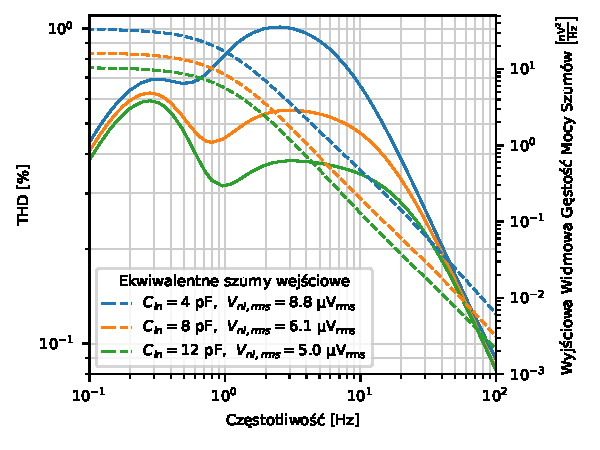
\includegraphics[scale=0.8]{scripts/tmp/thd_C_in.pdf} 
    \end{figure}
\end{columns}

\end{frame}


\part{Operacyjny wzmacniacz transkonduktancyjny}
% \begin{frame}{Implementacja teleskopowej kaskody ze zintegrowanym sprzężeniem AC}
%     \begin{columns}

%         \column{.6\textwidth}
%         \begin{figure}[H]
%             \includegraphics[scale = 0.75]{ch4/chap4Scheme.pdf} 
%         \end{figure}

%         \column{.35\textwidth}


%         \begin{block}{Kluczowe wymagnia}
%         \begin{itemize}
%             \item optymalizacja szumowa
%             \item powierzchnia
%             \item pobór mocy
%         \end{itemize}
%             \end{block}



%     \end{columns}   
%  \end{frame}



% \begin{frame}{Analiza szumowa pary różnicowej}
%     \begin{figure}[H]
%         \centering
%         \includegraphics[scale = 0.75]{scripts/tmp/differentialPair.pdf}  
%     \end{figure}

% \end{frame}



\begin{frame}{Przedwzmacniacz z wejściowym obwodem sprzęgającym AC}
    \begin{columns}

    \column{.65\textwidth}
    \begin{figure}[H]
        \centering
        \includegraphics[scale=0.45]{ch4/channel.pdf} 
    \end{figure}   

    \column{.35\textwidth}

    \begin{block}{
    }
    {\renewcommand\normalsize{\small}%
    \normalsize
    \begin{itemize}
        \item Konfiguracja  teleskopowej kaskody  jako aktywny OTA
        \item Polaryzacja pary różnicowej w obszarze podprogowym pracy tranzystora
        \item  Napięcie zasilania $\SI{\pm 1.8}{\volt}$
    \end{itemize}
    \vspace{-1em}
    \begin{table}[H]
        \centering
        \begin{tabular}{lll} 
        \toprule
        \begin{tabular}[c]{@{}l@{}}Kluczowe \\tranzystory\end{tabular} & $W$ [$\SI{}{\micro\metre}$] & $L$ [$\SI{}{\micro\metre}$]  \\ 
        \toprule
        $M_{bias}$                                                       & 10                          & 10                           \\
        $M_1,\ M_2$                                                    & 300                         & 1                            \\
        $M_3,\ M_4$                                                    & 20                          & 2                            \\
        $M_5,\ M_6$                                                    & 5                           & 5                            \\
        $M_7,\ M_8$                                                    & 4                           & 48                           \\
        \bottomrule
        \end{tabular}
    \end{table}
    }
    \end{block}
    \end{columns}   
  
\end{frame}


% \begin{frame}{Blok korekcji}
% \begin{columns}

%     \column{.35\textwidth}
%     \begin{block}{
%         Projekt kanału}
%         \begin{figure}[H]
%             \centering
%             \includegraphics[scale = 0.4]{ch4/chap4Scheme.pdf}
%         \end{figure} 
%         \end{block}

%         \begin{block}{
%             Wyzwania do rozwiązania}
%             \begin{figure}[H]
%                 \centering
%                 \includegraphics[scale = 0.6]{ch4/vgs_corr_sch.pdf} 
%             \end{figure}   
%             \end{block}



%     \column{.6\textwidth}
%     \begin{columns}
%     \column{.45\textwidth}

%     \begin{figure}[H]
%         \centering
%         \includegraphics[scale = 0.45]{scripts/tmp/analyseVgsTHD_1.pdf}
%     \end{figure} 
%     \column{.45\textwidth}
%     \begin{figure}[H]
%         \centering
%         \includegraphics[scale =0.45]{scripts/tmp/analyseVgsTHD_2.pdf}
%     \end{figure} 
%     \end{columns}   

%     \begin{columns}
%     \column{.45\textwidth}

%     \begin{figure}[H]
%         \centering
%         \includegraphics[scale = 0.4]{ch4/vgs_corr0.pdf}
%     \end{figure} 
%     \column{.45\textwidth}
%     \begin{figure}[H]
%         \centering
%         \includegraphics[scale = 0.4]{ch4/vgs_corr1.pdf}
%     \end{figure} 
%     \end{columns}   
% \end{columns}  
% \end{frame}


\begin{frame}{}
    \begin{columns}

    \column{.45\textwidth}
    \begin{block}{}
        {\renewcommand\normalsize{\small}%
        \normalsize
        \begin{itemize}
            \item 8 wersji przedwzmacniacza i 14 kanałów
            \item 4 wersje tranzystorów PMOS tworzących pseudo-rezystory  --  $W/L$: $2/40,\ 1/40,\ 2/20,\ 1/20\ \SI{}{\micro\metre / \micro\metre}$
            \item 2 konfiguracje pojemności -- $C_{in}/C_f = 4/200,\ 8/400\ \SI{}{\pico\farad}/\SI{}{\femto\farad}$
        \end{itemize}
        }
    \end{block}

\vspace{-1em}
    \begin{figure}[H]
        \centering
        \includegraphics[trim={0 12cm 0 0},clip, scale = 0.5]{ch4/layoutASIC.pdf} 
    \end{figure}   
    \column{.5\textwidth}

    \begin{block}{
Symulacje Post-Layout
    }

    \begin{figure}[H]
        \centering
        \includegraphics[scale = 0.45]{scripts/tranSchematicLayout/tranSchematicLayout.pdf}  
    \end{figure}
    \vspace{-5mm} %5mm vertical space
    \begin{figure}[H]
        \centering
        \includegraphics[scale = 0.45]{scripts/noiseContribution/noiseContributionOut.pdf}  
    \end{figure}
    \end{block}
    \end{columns}   
  
\end{frame}






\part{Weryfikacja elektroniczna i neurofizjologiczna układu scalonego HiFiNeuroPre}
\begin{frame}{Zaprojektowane komponenty systemu testowego}

%     \begin{figure}[H]
%         \centering
%         \begin{subfigure}[b]{0.65\textwidth}
%             \centering
%             \includegraphics[width=\textwidth]{ch5/IMG_3725.jpg}

%         \end{subfigure}
%         \hfill
%         \begin{subfigure}[b]{0.3\textwidth}
%             \centering
%             \includegraphics[width=\textwidth]{ch5/chip.jpg} 
%             \includegraphics[width=\textwidth]{ch5/asic_photo.jpg}
%         \end{subfigure}     

%    \end{figure}
\begin{columns}
    \column{.57\textwidth}
    \vspace{-1em}

    \begin{figure}[H]
    \centering
        \includegraphics[width=0.9\textwidth]{ch5/IMG_3725.jpg}
    \end{figure}

    \column{.4\textwidth}
\vspace{-1.5em}
    \begin{figure}[H]
    \centering
        \includegraphics[width=\textwidth]{ch5/inputfile_A0.01VPP_vibias0.0_ictrl290_corr100_0_ver02_101_par0_test_generator.png} 
        \includegraphics[width=0.9\textwidth]{ch5/asic_photo.jpg}

    \end{figure}
\end{columns}


\end{frame}


\begin{frame}{Przykładowe wyniki -- regulacja częstotliwości granicznej}

    \begin{figure}[H]
        \centering
        \begin{subfigure}[b]{0.485\textwidth}
            \centering
            \includegraphics[scale=0.8]{scripts/tmp/bodePlotFc_2.pdf}  

        \end{subfigure}
        % \hfill
        \begin{subfigure}[b]{0.485\textwidth}
            \centering
            \includegraphics[scale=0.8]{scripts/tmp/bodePlotFc_ictrl.pdf}

        \end{subfigure}     

    \end{figure}
    \vspace{-2em}
    \begin{block}{}
        \begin{itemize}
            \item Częstotliwość graniczna regulowana w zakresie od $\SIrange{0.1}{20}{\hertz}$ 
            \item Jednorodność kanałów 
        \end{itemize}
    \end{block}


\end{frame}

%  

% \begin{frame}{Pomiary zniekształceń harmonicznych -- wpływ korekty}

%     \begin{columns}

%         \column{.45\textwidth}
%         \begin{block}{Brak globalnej korekty}
%             \begin{figure}[H]
%                 \centering
%                 \includegraphics[scale = 0.85]{scripts/tmp/thdFreqCorr0_0.pdf} 
%             \end{figure}   
%         \end{block}

%         \column{.45\textwidth}

%         \begin{block}{Korekta globalna}
%             \begin{figure}[H]
%                 \centering
%                 \includegraphics[scale = 0.85]{scripts/tmp/thdFreqCorr100_0.pdf}
%             \end{figure}   
%         \end{block}
%     \end{columns}

% \end{frame}

\begin{frame}{Przykładowe wyniki -- pomiary zniekształceń}
    \begin{columns}

        \column{.45\textwidth}
        \vspace{-1em}
        \begin{block}{}
            \begin{itemize}
                \item Podobny protokół pomiarowy do symulacji -- amplituda sygnału sinusoidalnego: $\SI{10}{\milli\volt_{pp}}$
                \item Zmierzony poziom zniekształceń niższy niż w symulacjach
            \end{itemize}
        \end{block}
        \vspace{-1em}

            \begin{figure}[H]
                \centering
                \includegraphics[trim={0 0.25cm 0 0.25cm}, clip, scale = 0.75]{scripts/embc2021THD_size/embc2021THD_size_0_100.pdf}
            \end{figure}   

            
        \column{.52\textwidth}
        Różne częstotliwości granicznej dla wybranej konfiguracji przedwzmacniacza
        \begin{figure}[H]
            \centering
            \includegraphics[scale=0.75]{scripts/embc2021THD_fc/embc2021THD_fc.pdf}
        \end{figure}

\end{columns}

\end{frame}
        % \begin{block}{Drugi wariant przedwzmacniacza z większymi pojemnościami wejściowymi}


        %     \begin{figure}[H]
        %         \centering
        %         \includegraphics[trim={0 0.25cm 0 0.25cm}, clip, scale = 0.8]{scripts/embc2021THD_size/embc2021THD_size_1_100.pdf}
        %     \end{figure}   
        % \end{block}
  

    % \begin{figure}[H]
    %     \centering
    %     \begin{subfigure}{0.485\textwidth}
    %         \centering
    %         \includegraphics[trim={0 0.25cm 0 0.25cm}, clip, scale = 0.6]{scripts/embc2021THD_size/embc2021THD_size_0_0.pdf}
    %     \end{subfigure}
    %     % \hfill
    %     \begin{subfigure}{0.485\textwidth}
    %         \centering
    %         \includegraphics[trim={0 0.25cm 0 0.25cm}, clip, scale = 0.6]{scripts/embc2021THD_size/embc2021THD_size_1_0.pdf}
    %     \end{subfigure} 
    %     % \vfill
    %     \begin{subfigure}{0.485\textwidth}
    %         \centering
    %         \includegraphics[trim={0 0.25cm 0 0.25cm}, clip, scale = 0.6]{scripts/embc2021THD_size/embc2021THD_size_0_100.pdf}
    %     \end{subfigure}
    %     % \hfill
    %     \begin{subfigure}{0.485\textwidth}
    %         \centering
    %         \includegraphics[trim={0 0.25cm 0 0.25cm}, clip, scale = 0.6]{scripts/embc2021THD_size/embc2021THD_size_1_100.pdf}
    %     \end{subfigure}   
    % \end{figure}


% \begin{frame}{Pomiary szumów}
%     % \begin{figure}[H]
%     %     \centering 
%     %     \includegraphics[scale=0.4]{scripts/tmp/measurementNoiseDataset.pdf}  
%     % \end{figure}

%     \begin{figure}[H]
%         \centering
%         \begin{subfigure}[b]{0.485\textwidth}
%             \centering
%             \includegraphics{scripts/tmp/noiseGND_in.pdf}
%         \end{subfigure}
%         % \hfill
%         \begin{subfigure}[b]{0.485\textwidth}
%             \centering
%             \includegraphics{scripts/tmp/noiseElektrodaNaCl.pdf}
%         \end{subfigure}     
%     \end{figure}
% \end{frame}



\begin{frame}{Eksperyment neurobiologiczny z wykorzystaniem systemu pomiarowego}
    \begin{columns}

        \column{.45\textwidth}
        \begin{figure}[H]
            \centering 
            \includegraphics[scale=0.175]{ch6/setupIBDtot.png}  
            \caption{Schemat stanowiska pomiarowego do celów eksperymentu neurobiologicznego w Instytucie Biologii Doświadczalnej PAN}
        \end{figure}

        \column{.53\textwidth}
        \vspace{-1em}

        \begin{block}{}
            \begin{itemize}
                \item Sonda komercyjna firmy Neuronexus -- 16 elektrod na trzpieniu sondy
                \item Wymuszona aktywność: Sonda w obszarze kory mózgowej na głębokości $\SI{1.4}{\milli\metre}$ pod powierzchnią mózgu
                \item Spontaniczna aktywność: Sonda w obszarze wzgórza a głębokości $\SI{6}{\milli\metre}$ pod powierzchnią mózgu
            \end{itemize}
        \end{block}
        \vspace{-1em}

        \begin{figure}[H]
            \centering 
            \includegraphics[scale=0.08]{ch6/tissueDescription.png}  
        \end{figure}
    \end{columns}

\end{frame}

% \begin{frame}{}
%     \begin{figure}[H]
%        % \begin{subfigure}{0.3\textwidth}
   
%        %  \end{subfigure}
%        %      \hfill
   
%        \begin{subfigure}{0.25\textwidth}
%            \includegraphics[scale = 0.75]{ch6/meaLFPnexus.pdf}
%             % \vfill
%         \end{subfigure}
%        % \hfill
%            \hspace{-5em}
%         \begin{subfigure}{0.7\textwidth}
%            \includegraphics[scale = 0.75]{scripts/tmp/signal_MEA_LFP_wide.pdf}
%         \end{subfigure}
%    \end{figure}
% \end{frame}

\begin{frame}{Aktywność neuronalna zarejestrowana przez HiFiNeuroPre}
    \begin{columns}
        \column{.6\textwidth}
            \vspace{-1em}

            \begin{block}{}
                {\renewcommand\normalsize{\small}%
                \normalsize
                \begin{itemize}
                    \item Stymulacja zewnętrzna aplikowana cyklicznie w różnych odstępach czasu -- od $\SIrange{3}{5}{\second}$;
                    \item 60 powtórzeń stymulacji w danym cyklu pomiarowym 
                    \item Kilka cykli pomiarowych dla różnych ustawień sprzętu
        
                \end{itemize}
                }
                \vspace{-1em}
                \begin{figure}[H]
                    % \begin{subfigure}{0.3\textwidth}
                
                    %  \end{subfigure}
                    %      \hfill
                
                    \begin{subfigure}{0.25\textwidth}
                        \includegraphics[scale = 0.45]{ch6/meaLFPnexus.pdf}
                        % \vfill
                    \end{subfigure}
                    % \hfill
                        \hspace{-2em}
                    \begin{subfigure}{0.7\textwidth}
                        \includegraphics[scale = 0.45]{scripts/tmp/signal_MEA_LFP_wide.pdf}
                    \end{subfigure}
                \end{figure}
            \end{block}
        \column{.35\textwidth}
        \vspace{-1em}

        \begin{block}{Zapis spontanicznej aktywności neuronalnej}
            \begin{figure}[H]
                \centering
                \includegraphics[scale=0.6]{scripts/tmp/signal_MEA_AP_2.pdf}
        \end{figure}
        \end{block}

    \end{columns}
        

    % \begin{figure}[H]
    %     \centering
    %     \begin{subfigure}[b]{0.485\textwidth}
    %         \centering
    %         \includegraphics[scale=0.8]{scripts/tmp/signal_MEA_AP_1.pdf}
    %         \caption{}
    %     \end{subfigure}
    %     % \hfill
    %     \begin{subfigure}[b]{0.485\textwidth}
    %         \centering
    %         \includegraphics[scale=0.8]{scripts/tmp/signal_MEA_AP_2.pdf}
    %         \caption{}
    %     \end{subfigure}     
    % \end{figure}
\end{frame}


\part{Podsumowanie}
\begin{frame}{Podsumowanie testów elektronicznych}

\begin{longtblr}[
    caption = {Parametry przedwzmacniacza na podstawie pomiarów weryfikacyjnych}
    % label = {table:paramResult},
  ]{
    hline{1-2,11} = {-}{0.08em},
  }
  \textbf{Parametr}                                                                 & \textbf{Wartość}                    \\
  Napięcia zasilania                                                                & $\SI{\pm 1.8}{\volt}$               \\
  Całkowity prąd                                                                    & $\SI{2}{\micro\ampere}$             \\
  Pobór mocy dla pojedynczego kanału                                                & $\SI{7.2}{\micro\watt}$             \\
  Wzmocnienie z zamkniętą pętlą sprzężenia                                          & $\SI{25.9}{\deci\bel}$              \\
  Zakres dolnej częstotliwości granicznej                                           & $\SIrange{0.1}{20}{\hertz}$         \\
  Ekwiwalentny szum wejściowy w zakresie LFP                                        & $\SI{7.5}{\micro\volt_{rms}}$       \\
  Ekwiwalentny szum wejściowy w zakresie AP                                         & $\SI{6.7}{\micro\volt_{rms}}$       \\
  Zniekształcenia harmonioczne THD – $\SI{10}{\milli\volt_{pp}}\ \SI{1.68}{\hertz}$ & $\SI{0.94}{\percent}$               \\
  Pole powierzchni pojedynczego przedwzmacniacza                                    & $\SI{0.0071}{\milli\metre\squared}$ 
  \end{longtblr}
\end{frame}

\begin{frame}{Wnioski}
\begin{itemize}
    \item 	
\end{itemize}
\end{frame}
% % \ifdefined\textleftmargin
% 	%%%%%%%%%%%%%%%%
% 	\begin{frame}[fragile]{\iflanguage{polish}{Informacje}{Information}}
% 		\begin{center}
% 			\iflanguage{polish}{
% 				$\Longleftarrow$ Aktualna wartość \hfill Aktualna wartość $\Longrightarrow$\\
% 				$\Longleftarrow$ rozmiaru lewego marginesu \hfill rozmiaru prawego marginesu $\Longrightarrow$\\
% 				$\Longleftarrow$ to \the\textleftmargin \hfill to \the\textrightmargin $\Longrightarrow$
% 			}{
% 				$\Longleftarrow$ The current value of \hfill The current value of $\Longrightarrow$\\
% 				$\Longleftarrow$ the  left  margin size \hfill the right margin size $\Longrightarrow$\\
% 				$\Longleftarrow$ is \the\textleftmargin \hfill is \the\textrightmargin $\Longrightarrow$
% 			}
% 		\end{center}
% 		\iflanguage{polish}{
% 			Możesz je zmieniać za pomocą parametru 'margins' \pauza
% 		}{
% 			You can change them with the 'margins' parameter ---
% 		}
% 		\verb+\usetheme[margins=...]{AGH}+
% 	\end{frame}
% \fi
%%%%%%%%%%%%%%%%

%%%%%%%%%%%%%%%%
\begin{frame}{\iflanguage{polish}{Plan prezentacji}{Outline}}
	\tableofcontents[pausesections]
\end{frame}
%%%%%%%%%%%%%%%%
\section{\iflanguage{polish}{Elementy podstawowe}{Basic elements}}
%%%%%%%%%%%%%%%%
\begin{frame}{\iflanguage{polish}{Wyszczególnienie}{Itemize}}
	\begin{columns}
		\column{0.5\textwidth}
		\begin{itemize}
			\item \iflanguage{polish}{Element 1}{Item 1}
			\item \iflanguage{polish}{Element 2}{Item 2}
			\item \iflanguage{polish}{Element 3}{Item 3}
		\end{itemize}
		\column{0.5\textwidth}
		\pause
		\structure{\iflanguage{polish}{Odkrywanie po kolei}{Uncovering one by one}}
		\begin{itemize}[<+->]
			\item \iflanguage{polish}{Element 1}{Item 1}
			\item \iflanguage{polish}{Element 2}{Item 2}
			\item \iflanguage{polish}{Element 3}{Item 3}
		\end{itemize}
		\onslide
	\end{columns}
\end{frame}
%%%%%%%%%%%%%%%%
\begin{frame}{\iflanguage{polish}{Wyliczenie}{Enumerate}}
	\begin{columns}
		\column{0.5\textwidth}
		\begin{enumerate}
			\item \iflanguage{polish}{Element 1}{Item 1}
			\item \iflanguage{polish}{Element 2}{Item 2}
			\item \iflanguage{polish}{Element 3}{Item 3}
		\end{enumerate}
		\column{0.5\textwidth}
		\pause
		\structure{\iflanguage{polish}{Odkrywanie elementów po kolei z jednoczesnym wyróżnianiem}{Uncovering elements in turn with simultaneous highlighting}}
		\begin{enumerate}[<+-|alert@+>]
			\item \iflanguage{polish}{Element 1}{Item 1}
			\item \iflanguage{polish}{Element 2}{Item 2}
			\item \iflanguage{polish}{Element 3}{Item 3}
		\end{enumerate}
		\onslide
	\end{columns}
\end{frame}
%%%%%%%%%%%%%%%%
\section{\iflanguage{polish}{Matematyka}{Mathematics}}
%%%%%%%%%%%%%%%%
\begin{frame}{\iflanguage{polish}{Podstawowe bloki}{Basic blocks}}
	% Examples from "The beamer class User Guide"
	\iflanguage{polish}{
		\begin{block}{Definicja}
			\alert{Zbiór} składa się z elementów.
		\end{block}
		\begin{exampleblock}{Przykład}
			Zbiór $\{1,2,3,5\}$ zawiera cztery elementy.
		\end{exampleblock}
		\begin{alertblock}{Błędne Twierdzenie}
			$1=2$.
		\end{alertblock}
	}{
		\begin{block}{Definition}
			A \alert{set} consists of elements.
		\end{block}
		\begin{exampleblock}{Example}
			The set $\{1,2,3,5\}$ has four elements.
		\end{exampleblock}
		\begin{alertblock}{Wrong Theorem}
			$1=2$.
		\end{alertblock}
	}
\end{frame}
%%%%%%%%%%%%%%%%
\begin{frame}{\iflanguage{polish}{Otoczenia matematyczne}{Math environments}}
	\begin{columns}
		\column{0.45\textwidth} %The first column
		\structure{\iflanguage{polish}{Twierdzenia}{Theorems}}
		\begin{theorem}[\iflanguage{polish}{Pitagorasa}{Pythagorean}]
			$a^{2}+  b^{2}=  c^{2}$
		\end{theorem}
		\column{0.45\textwidth} %The second column
		\structure{\iflanguage{polish}{Dowody}{Proofs}}
		\begin{proof}
			\ldots
		\end{proof}
	\end{columns}
	\vfill
	\ldots
	\vfill
	\begin{definition}
		\ldots
	\end{definition}
\end{frame}
%%%%%%%%%%%%%%%%
\begin{frame}{\iflanguage{polish}{Dynamiczny wzór matematyczny}{Dynamic mathematical formula}}
	\[
		\binom{n}{k} = \pause \frac{n!}{k!(n-k)!}
	\]
\end{frame}
%%%%%%%%%%%%%%%%
% \section{\iflanguage{polish}{Informatyka}{Computer Science}}
% %%%%%%%%%%%%%%%%
% \subsection*{\iflanguage{polish}{Wstawianie kodów źródłowych}{Inserting source codes}}
% %%%%%%%%%%%%%%%%
% \begin{frame}[fragile]{\iflanguage{polish}{Użycie otoczenia 'listings'}{Using the 'listings' environment}}
% 	\begin{lstlisting}[language=C++]
% /* The first  program in C++ */  %*\pause*)
% #include <iostream>  %*\pause*)
% using namespace std; %*\pause*)
% void main() 
% {       %*\pause*)
%   cout %*\pause*) << "Hello World!"%*\pause*) << endl; %*\onslide<4->*)
% } %*\onslide*)
% \end{lstlisting}
% \end{frame}
%%%%%%%%%%%%%%%%
% \begin{frame}[fragile]{\iflanguage{polish}{Użycie otoczenia 'minted'}{Using the 'minted' environment}}
% 	\begin{minted}[beameroverlays,escapeinside=||]{C++}
% /* The first  program in C++ */  |\pause|
% #include <iostream>  |\pause|
% using namespace std; |\pause|
% void main() 
% {       |\pause|
%   cout |\pause| << "Hello World!"|\pause| << endl; |\onslide<4->|
% } |\onslide|
% 	\end{minted}
% \end{frame}
% %%%%%%%%%%%%%%%%%%%%%%%
% \appendix
% %%%%%%%%%%%%%%%%%%%%%%%
% \begin{frame}[allowframebreaks]{\iflanguage{polish}{Bibliografia}{Bibliography}}
% 	\begin{thebibliography}{9}
% 		\setbeamertemplate{bibliography item}[online]
% 		\bibitem{wikibook}{Wikibooks \newblock \LaTeX/Source Code Listings \newblock \url{https://en.wikibooks.org/wiki/LaTeX/Source_Code_Listings}}
% 		\bibitem{beamer}{Till Tantau, Joseph Wright, Vedran Miletić \newblock The beamer class \newblock \url{http://mirror.ctan.org/macros/latex/contrib/beamer/doc/beameruserguide.pdf}}
% 		\setbeamertemplate{bibliography item}[book]
% 		\bibitem{lamport}{Leslie Lamport \newblock LATEX: a document preparation system : user's guide and reference manual \newblock Addison-Wesley Pub. Co., 1994 }
% 		\setbeamertemplate{bibliography item}[article]
% 		\iflanguage{polish}{
% 			\bibitem{article1}{Autor \newblock Tytuł artykułu \newblock Edytor, rok \newblock Uwagi}
% 			\setbeamertemplate{bibliography item}[triangle]
% 			\bibitem{article2}{Autor \newblock Tytuł artykułu \newblock Edytor, rok \newblock Uwagi}
% 			\setbeamertemplate{bibliography item}[text]
% 			\bibitem{article3}{Autor \newblock Tytuł artykułu \newblock Edytor, rok \newblock Uwagi}
% 			\bibitem[Polak98]{article4}{Autor \newblock Tytuł artykułu \newblock Edytor, rok \newblock Uwagi}
% 		}{
% 			\bibitem{article1}{Author \newblock Title of the article\newblock Editor, year \newblock Notes}
% 			\setbeamertemplate{bibliography item}[triangle]
% 			\bibitem{article2}{Author \newblock Title of the article\newblock Editor, year \newblock Notes}
% 			\setbeamertemplate{bibliography item}[text]
% 			\bibitem{article3}{Author \newblock Title of the article\newblock Editor, year \newblock Notes}
% 			\bibitem[Polak98]{article4}{Author \newblock Title of the article\newblock Editor, year \newblock Notes}
% 		}
% 	\end{thebibliography}
% \end{frame}
\end{document}
